\subsection{三角形、梯形的中位线}\label{subsec:czjh1-4-11}

\begin{enhancedline}

连结三角形两边中点的线段叫做\zhongdian{三角形的中位线}。

注意:三角形的中位线和三角形的中线不同。

\begin{dingli}[三角形中位线定理]
    三角形的中位线平行于第三边,并且等于它的一半。
\end{dingli}

\begin{wrapfigure}[8]{r}{5cm}
    \centering
    \begin{tikzpicture}
    \tkzDefPoints{0/0/B, 3/0/C, 2.3/3/A}
    \tkzDefMidPoint(A,B)  \tkzGetPoint{D}
    \tkzDefMidPoint(A,C)  \tkzGetPoint{E}
    \tkzDefPointOnLine[pos=2](D,E)  \tkzGetPoint{F}
    \tkzDrawPolygon(A,B,C)
    \tkzDrawSegments(D,E)
    \tkzDrawSegments[dashed](E,F  F,C)
    \tkzLabelPoints[above](A)
    \tkzLabelPoints[left](B,D)
    \tkzLabelPoints[right](F)
    \tkzLabelPoints[above right](E)
    \tkzLabelPoints[below](C)
\end{tikzpicture}


    \caption{}\label{fig:czjh1-4-46}
\end{wrapfigure}

已知: $\triangle ABC$ 中, $AD = DB$, $AE = EC$(图 \ref{fig:czjh1-4-46})。

求证:$DE \pingxing BC$, $DE = \exdfrac{1}{2} BC$。

\zhengming 延长 $DE$ 至点 $F$, 使 $EF = DE$, 连结 $CF$。

$\because$ \quad $AE = EC$, $DE = EF$,

$\therefore$ \quad 点 $A$ 与 $C$, $D$ 与 $F$ 关于点 $E$ 对称。

$\therefore$ \quad $AD \pxqdy FC$ (中心对称的性质)。

又 $\because$ \quad $AD = DB$,

$\therefore$ \quad $DB \pxqdy FC$。

$\therefore$ \quad 四边形 $BCFD$ 是平行四边形。

$\therefore$ \quad $DF = BC$, $DE \pingxing BC$ (平行四边形的对边平行且相等)。

$\because$ \quad $DE = \exdfrac{1}{2} DF$,

$\therefore$ \quad $DE = \exdfrac{1}{2} BC$。


连结梯形两腰中点的线段叫做\zhongdian{梯形的中位线}。

\begin{dingli}[梯形中位线定理]
    梯形的中位线平行于两底,并且等于两底和的一半。
\end{dingli}


% \begin{figure}[htbp]
%     \centering
%     \begin{minipage}[b]{5cm}
%         \centering
%         \begin{tikzpicture}
    \tkzDefPoints{0/0/B, 3/0/C, 2.3/3/A}
    \tkzDefMidPoint(A,B)  \tkzGetPoint{D}
    \tkzDefMidPoint(A,C)  \tkzGetPoint{E}
    \tkzDefPointOnLine[pos=2](D,E)  \tkzGetPoint{F}
    \tkzDrawPolygon(A,B,C)
    \tkzDrawSegments(D,E)
    \tkzDrawSegments[dashed](E,F  F,C)
    \tkzLabelPoints[above](A)
    \tkzLabelPoints[left](B,D)
    \tkzLabelPoints[right](F)
    \tkzLabelPoints[above right](E)
    \tkzLabelPoints[below](C)
\end{tikzpicture}


%         \caption{}\label{fig:czjh1-4-46}
%     \end{minipage}
%     \qquad
%     \begin{minipage}[b]{5cm}
%         \centering
%         \begin{tikzpicture}
    \tkzDefPoints{0/0/B, 3/0/C, 1.2/2.5/A, 2.5/2.5/D}
    \tkzDefMidPoint(A,B)  \tkzGetPoint{M}
    \tkzDefMidPoint(D,C)  \tkzGetPoint{N}
    \tkzInterLL(A,N)(B,C)  \tkzGetPoint{E}
    \tkzDrawPolygon(A,B,C,D)
    \tkzDrawSegment(M,N)
    \tkzDrawSegments[dashed](A,E  C,E)
    \tkzLabelPoints[left](A,B,M)
    \tkzLabelPoints[right](D,N,E)
    \tkzLabelPoints[below](C)
\end{tikzpicture}


%         \caption{}\label{fig:czjh1-4-47}
%     \end{minipage}
% \end{figure}


已知:梯形 $ABCD$ 中,$AD \pingxing BC$, $AM = MB$, $DN = NC$ (图 \ref{fig:czjh1-4-47})。

\begin{wrapfigure}[8]{r}{5cm}
    \centering
    \begin{tikzpicture}
    \tkzDefPoints{0/0/B, 3/0/C, 1.2/2.5/A, 2.5/2.5/D}
    \tkzDefMidPoint(A,B)  \tkzGetPoint{M}
    \tkzDefMidPoint(D,C)  \tkzGetPoint{N}
    \tkzInterLL(A,N)(B,C)  \tkzGetPoint{E}
    \tkzDrawPolygon(A,B,C,D)
    \tkzDrawSegment(M,N)
    \tkzDrawSegments[dashed](A,E  C,E)
    \tkzLabelPoints[left](A,B,M)
    \tkzLabelPoints[right](D,N,E)
    \tkzLabelPoints[below](C)
\end{tikzpicture}


    \caption{}\label{fig:czjh1-4-47}
\end{wrapfigure}

求证: $MN \pingxing BC$, $MN = \exdfrac{1}{2} (AD + BC)$。

分析: 我们设法利用三角形中位线定理。 连结 $AN$ 并延长,可得 $\triangle ABE$,
如果能证明 $N$ 是 $AE$ 的中点,那么就容易证明这个定理了。

\zhengming 连结 $AN$ 并延长,交 $BC$ 的延长线于点 $E$。

$\because$ \quad $DN = NC$, $AD \pingxing CE$,

$\therefore$ \quad $AN = NE$ (平行线等分线段定理)。

在 $\triangle ABE$ 中,

$\because$ \quad $AM = MB$, $AN = NE$,

$\therefore$ \quad $MN \pingxing BE$, $MN = \exdfrac{1}{2} (BC + CE)$ (三角形中位线定理)。

又 $\because$ \quad 点 $D$ 与 $C$, 点 $A$ 与 $E$ 关于点 $N$ 对称,

$\therefore$ \quad $AD = CE$。

$\therefore$ \quad $MN = \exdfrac{1}{2} (AD + BC)$。



\liti[0] 求证顺次连结四边形四条边的中点,所得的四边形是平行四边形。

已知: 如图 \ref{fig:czjh1-4-48}, 在四边形 $ABCD$ 中,$E$、$F$、$G$、$H$ 分别是 $AB$、$BC$、$CD$、$DA$ 的中点。

求证:四边形 $EFGH$ 是平行四边形。

\zhengming 连结 $AC$。

$\because$ \quad $AH = HD$, $CG = GD$,

$\therefore$ \quad $HG \pingxing AC$, $HG = \exdfrac{1}{2} AC$ (三角形中位线定理)。

同理 $EF \pingxing AC$, $EF = \exdfrac{1}{2} AC$。

$\therefore$ \quad $HG \pxqdy EF$。

所以四边形 $EFGH$ 是平行四边形。

\begin{figure}[htbp]
    \centering
    \begin{minipage}[b]{5cm}
        \centering
        \begin{tikzpicture}
    \tkzDefPoints{0/0/B, 3/0/C, 0.6/1.5/A, 2.6/2.2/D}
    \tkzDefMidPoint(A,B)  \tkzGetPoint{E}
    \tkzDefMidPoint(B,C)  \tkzGetPoint{F}
    \tkzDefMidPoint(C,D)  \tkzGetPoint{G}
    \tkzDefMidPoint(D,A)  \tkzGetPoint{H}
    \tkzDrawPolygon(A,B,C,D)
    \tkzDrawPolygon(E,F,G,H)
    \tkzDrawSegments[dashed](A,C)
    \tkzLabelPoints[left](A,B,E)
    \tkzLabelPoints[right](C,G,D)
    \tkzLabelPoints[below](F)
    \tkzLabelPoints[above](H)
\end{tikzpicture}


        \caption{}\label{fig:czjh1-4-48}
    \end{minipage}
    \qquad
    \begin{minipage}[b]{5cm}
        \centering
        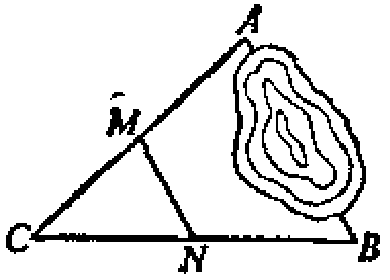
\includegraphics[width=4.0cm]{../pic/czjh1-ch4-subsec11-lx-01.png}
        \caption*{(第 1 题)}
    \end{minipage}
\end{figure}

\begin{lianxi}

\xiaoti{(口答) $A$、$B$ 两点被池塘隔开,在 $AB$ 外选一点 $C$,
    连结 $AC$ 和 $BC$,并分别找出 $AC$ 和 $BC$ 的中点 $M$、$N$。
    如果测得 $MN = 20\;\mi$, 那么 $A$、 $B$ 两点间的距离是多少? 为什么?
}

\xiaoti{已知: 三角形的各边分别为 $6\;\limi$、 $8\;\limi$ 和 $10\;\limi$,
    求连结各边中点所成三角形各边的长。
}

\xiaoti{已知: 梯形 $ABCD$, $AD \pingxing BC$, 对角钱 $AC$、$BD$ 相交于点 $O$,
    $A'$、$B'$、$C'$、$D'$ 分别是 $AO$、$BO$、$CO$、$DO$ 的中点。求证:
}
\begin{xiaoxiaotis}

    \xxt{四边形 $A'B'C'D'$ 是梯形;}

    \xxt{梯形 $ABCD$ 的周长等于梯形 $A'B'C'D'$ 周长的 2 倍。}

\end{xiaoxiaotis}


\xiaoti{}%
\begin{xiaoxiaotis}%
    \xxt[\xxtsep]{梯形的上底长 $8\;\limi$, 下底长 $9\;\limi$, 求中位线长;}

    \xxt{梯形的上底长 $8\;\limi$, 中位线长 $9\;\limi$, 求下底长。}

\end{xiaoxiaotis}

\end{lianxi}
\end{enhancedline}

